\lab{Algorithms}{Scientific Visualization}{Scientific Visualization}

\objective{Go over techniques for making publication ready figures and making other pretty things.}

Python and SciPy have no built-in plotting capabilities.  These capabilities are provided by Matplotlib.  In this lab we will be focusing on producing publication quality figures in Matplotlib using Python and SciPy.  Thus far we have produced many different plots for several applications.  Here we will focus on different ways of presenting those plots so that they are more informative and aesthetically pleasing.

\section{The \li{pyplot.plot} Command}  
Several of the past labs have required the use of the \li{pyplot.plot} command.  While what we have done so far as been fairly straightforward as far as plotting is concerned, a quick glance at the Matplotlib documentation for \li{pyplot.plot} reveals a plethora of options that can be set to adjust the final plot.

How we use the \li{pyplot.plot} command will vary with our application.  Plotting data requires a very different presentation approach than graphing straight lines.  In the sequel we examine several different options.

\begin{table}[h!]
\begin{center}
	\begin{tabular}{|c|c|}
	
	\hline
	
	Usage & Property Options\\
	
	\hline
	
	\li{color} & \li{yellow, green, blue} etc., or user defined colors \\& given by $[r g b]$, a three element red, green, \\& blue vector.  See documentation for full list. \\
	
	\hline
	
	\li{linestyle} & \li{-, --, :, -., 'None'} \\
	
	\hline
	
	\li{linewidth} & Width in points.  $1$ point is $\frac{1}{72}$ inch.  Default is $1.0$ points. \\
	
	\hline
	
	\li{marker} & \li{+, *, x, .} etc. See documentation for full list. \\
	
	\hline
	\end{tabular}
\end{center}
\caption{Common Plot commands in MATLAB}
\end{table}

For example, if we wanted to plot $f(x) = x^2$, we don't need to extend our typical plotting knowledge much, except maybe we like green better than blue:

\begin{lstlisting}[style=python]
: import matplotlib.pyplot as plt
: import scipy as sp
: x = sp.linspace(-1,5,50)
: f = lambda x: x**2
: plt.plot(x, map(f, x), color='green')
: plt.show()
\end{lstlisting}

See figure 37.1.

\begin{figure}
\begin{center}
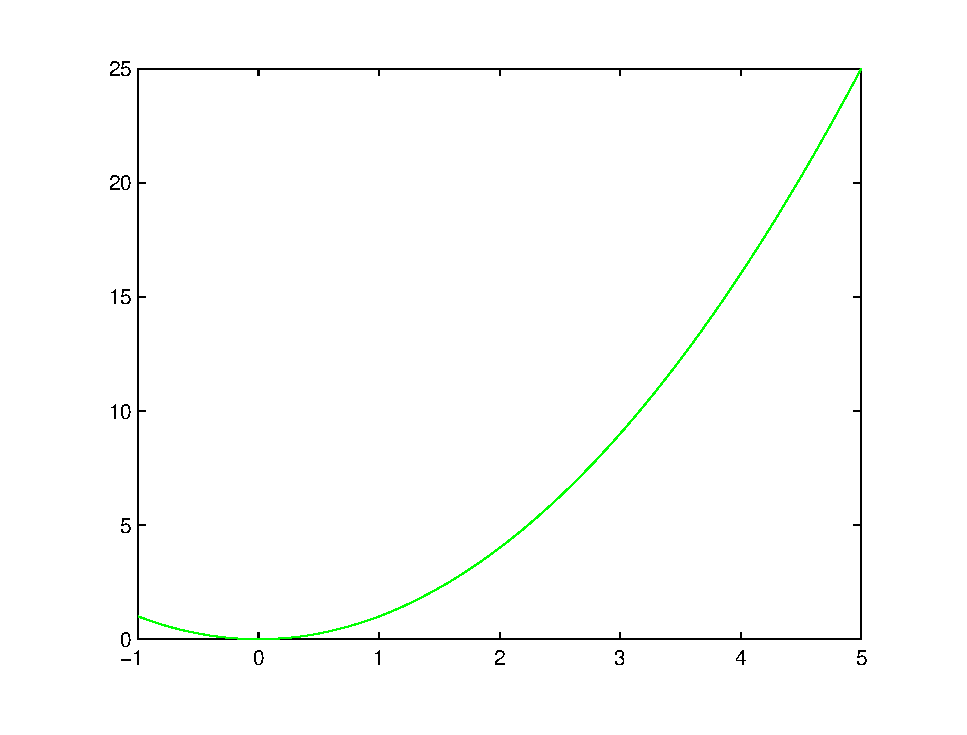
\includegraphics[scale=0.5]{./FiguresMAT/plot1}
\caption{Graph of $f(x) = x^2$}
\end{center}
\end{figure}


However, if we wanted to plot the data drawn from a certain distribution, we would want to use the plot command in a very different way.  For example:

%Explain the code?
\begin{lstlisting}[style=python]
>> X = random('Normal',0,1,[100,1]);
>> plot(X,'marker','*','LineStyle','none');
\end{lstlisting}

See figure 37.2.

\begin{figure}
\begin{center}
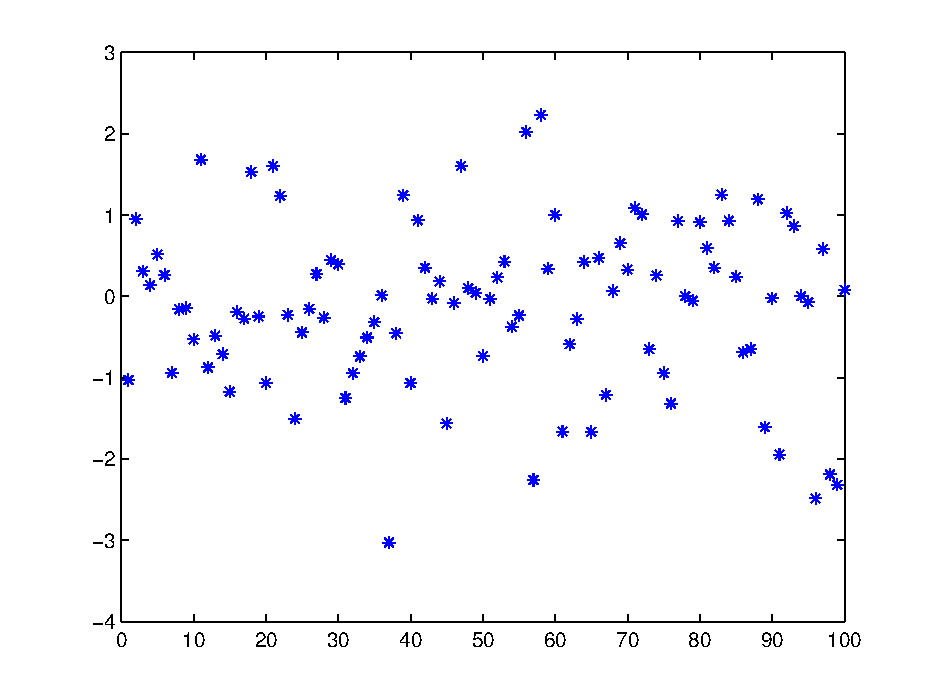
\includegraphics[scale=0.5]{./FiguresMAT/plot3}
\caption{100 data points pulled from a normal distribution}
\end{center}
\end{figure}

The \li{hold} command will also be useful for when plotting more than one graph on a single plot.  For example, if we wanted to graph $f(x) = \sin{x}$ and it's derivative $f'(x) = \cos{x}$, we would do the following:

\begin{lstlisting}[style=python]
: f = lambda x: sp.sin(x)
: df = lambda x: sp.cos(x)
: x = sp.linspace(0,2*sp.pi, 50)
: plt.hold(True)
: plot(x, map(f, x), color='blue')
: plot(x, map(df, x), color='green')
: plt.hold(False)
: plt.show()
\end{lstlisting}

See figure 37.3.

\begin{figure}
\begin{center}
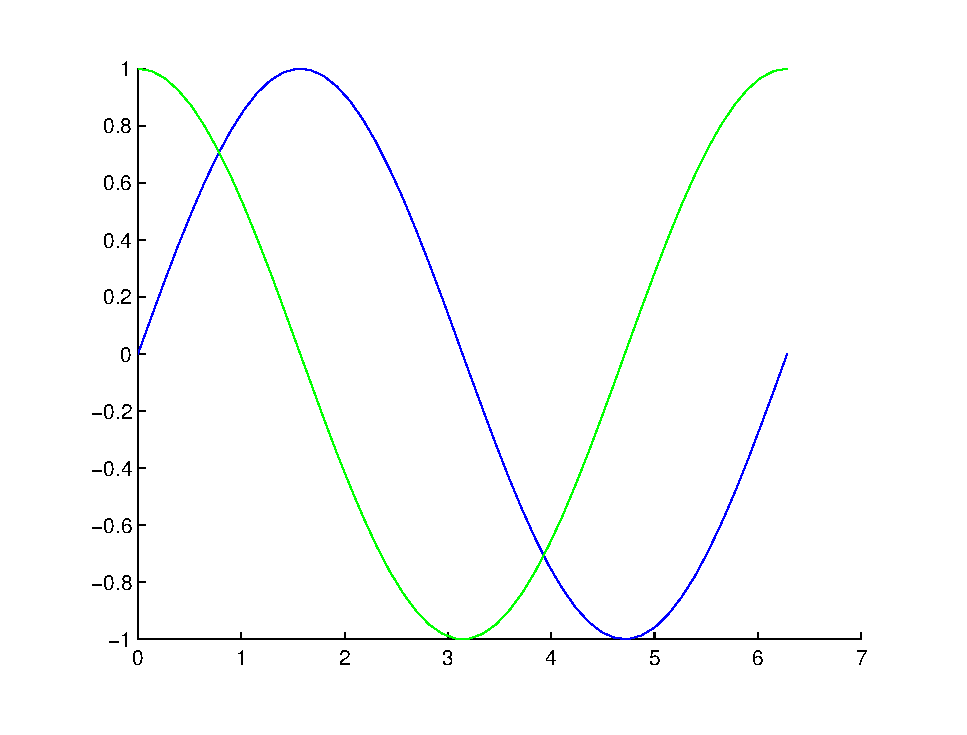
\includegraphics[scale=0.5]{./FiguresMAT/plot2}
\caption{$f(x) = \sin{x}$ and $f'(x) = \cos{x}$. Note the color choice makes for better presentation.}
\end{center}
\end{figure}

\begin{problem}  Using the MATLAB documentation and the aforementioned commands, do the following:
\begin{itemize}
\item Generate 25 data points from a distribution of your choosing.  Plot the data points and the least squares regression line on the same plot.  Use different colors and symbols for the data and the regression line.
\item 
\end{itemize}
\end{problem}

\subsection{Changing the Plot window}

Within in MATLAB we have several options for changing the \li{plot} window.  This includes adding captions and other labels, legends, and altering the axes (among other things).  For example, we plot 3 trajectories of a projectile shot from a cannon at 30 meters per second.

\begin{lstlisting}[style=python]
: g = 9.8
: v = 30.0
: t = linspace(0,6,100)
:
: h1 = lambda t: v*sp.math.sin(sp.pi/6)*t-0.5*g*t**2
: h2 = lambda t: v*sp.math.sin(sp.pi/4)*t-0.5*g*t**2
: h3 = lambda t: v*sp.math.sin(sp.pi/3)*t-0.5*g*t**2
:
: plt.hold(True)
: plt.plot(v*sp.math.cos(sp.pi/6)*t, map(h1, t), color='green')
: plt.plot(v*sp.math.cos(sp.pi/4)*t, map(h2, t), color='blue')
: plt.plot(v*sp.math.cos(sp.pi/3)*t, map(h3, t), color='red')
: plt.axis([0, 100, 0, 40])
: plt.xlabel('Distance')
: plt.ylabel('Height')
: plt.hold(False)
: plt.show()
\end{lstlisting}

See figure 37.4

\begin{figure}
\begin{center}
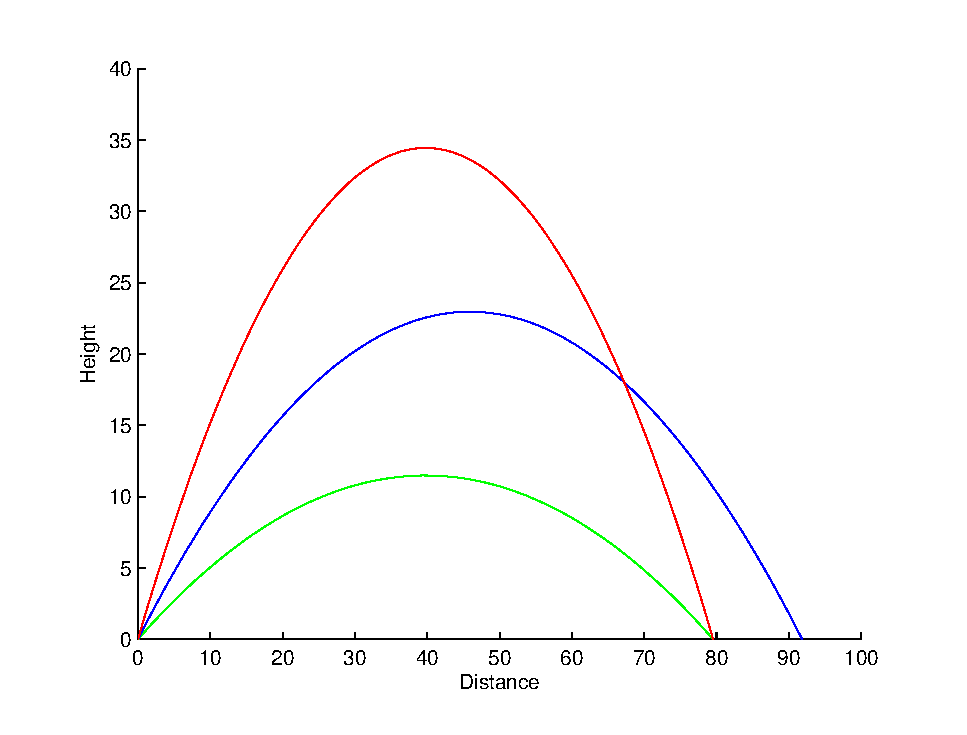
\includegraphics[scale=0.5]{./FiguresMAT/plot4}
\caption{Trajectory of a projectile fired at three different angles.}
\end{center}
\end{figure}

\begin{problem} 
\end{problem}

\section{The \li{subplot} command}  
Often times we want to include two or more plots in a single figure.  This is done using the \li{subplot} command.  This command will break the plot window into an $m\times n$ matrix of plots.  The subplot windows are numbered starting at $1$ in the top left cell and then ascending from left to right, top to bottom.  For example, instead of using different colors on the previous example, we could do 3 separate plots in a single window.  We could also include a graph of, for example, vertical velocity vs. time, which is informative but unable to be included in the same plot since it requires different units.  Let's see how this is done.

\begin{lstlisting}[style=python]
: g = 9.8
: v = 30.0
: t = linspace(0,6,100)
:
: h1 = lambda t: v*sp.math.sin(sp.pi/6)*t-0.5*g*t**2
: h2 = lambda t: v*sp.math.sin(sp.pi/4)*t-0.5*g*t**2
: h3 = lambda t: v*sp.math.sin(sp.pi/3)*t-0.5*g*t**2
:
: plt.subplot(221)
: plt.plot(v*cos(pi/6)*t,h1(t),'color','green')
: plt.axis([0, 100, 0, 40])
: plt.xlabel('Distance')
: plt.ylabel('Height')
: plt.title('30 degrees')
:
: plt.subplot(222)
: plt.plot(t, v*sin(pi/6) - g*t,'color','green')
: plt.xlabel('Time')
: plt.ylabel('Vertical Velocity')
:
: plt.subplot(223)
: plt.plot(v*cos(pi/4)*t,h2(t),'color','blue')
: plt.axis([0, 100, 0, 40])
: plt.xlabel('Distance')
: plt.ylabel('Height')
: plt.title('45 degrees')
:
: plt.subplot(224)
: plt.plot(t, v*sin(pi/4) - g*t, 'color','blue')
: plt.xlabel('Time')
: plt.ylabel('Vertical Velocity')
\end{lstlisting}

See figure 37.5.

\begin{figure}
\begin{center}
%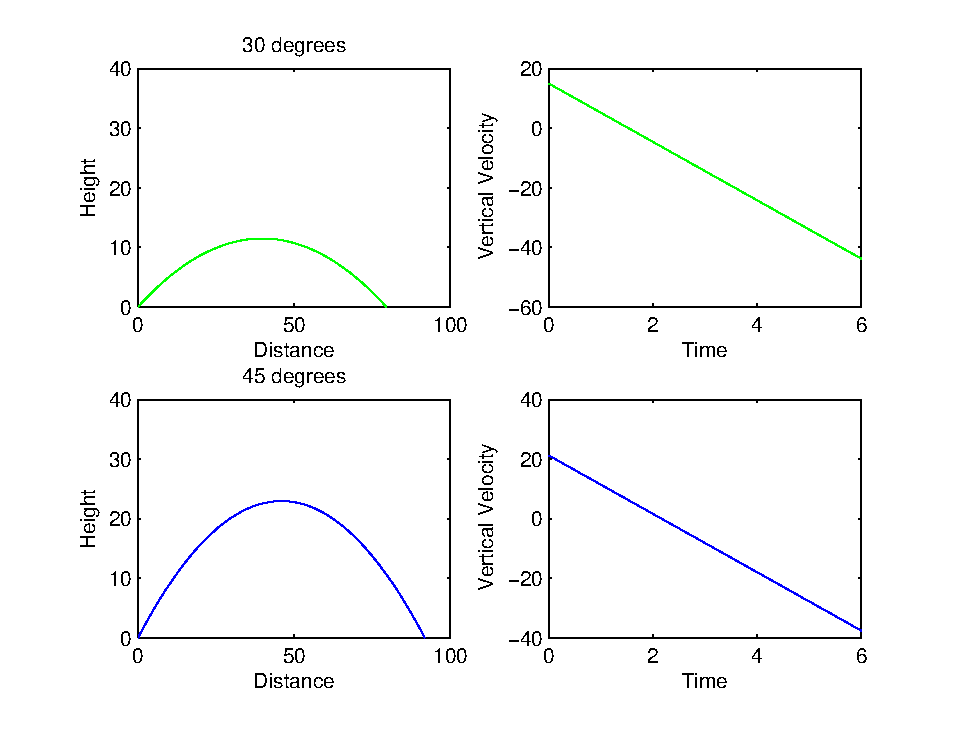
\includegraphics[scale=0.5]{./Figures/plot5}
\caption{Trajectory of a projectile fired at two different angles and the projectiles corresponding vertical velocity at time $t$.}
\end{center}
\end{figure}

\section{Time graphics?}



